\begin{figure}[t]
    \centering
    % 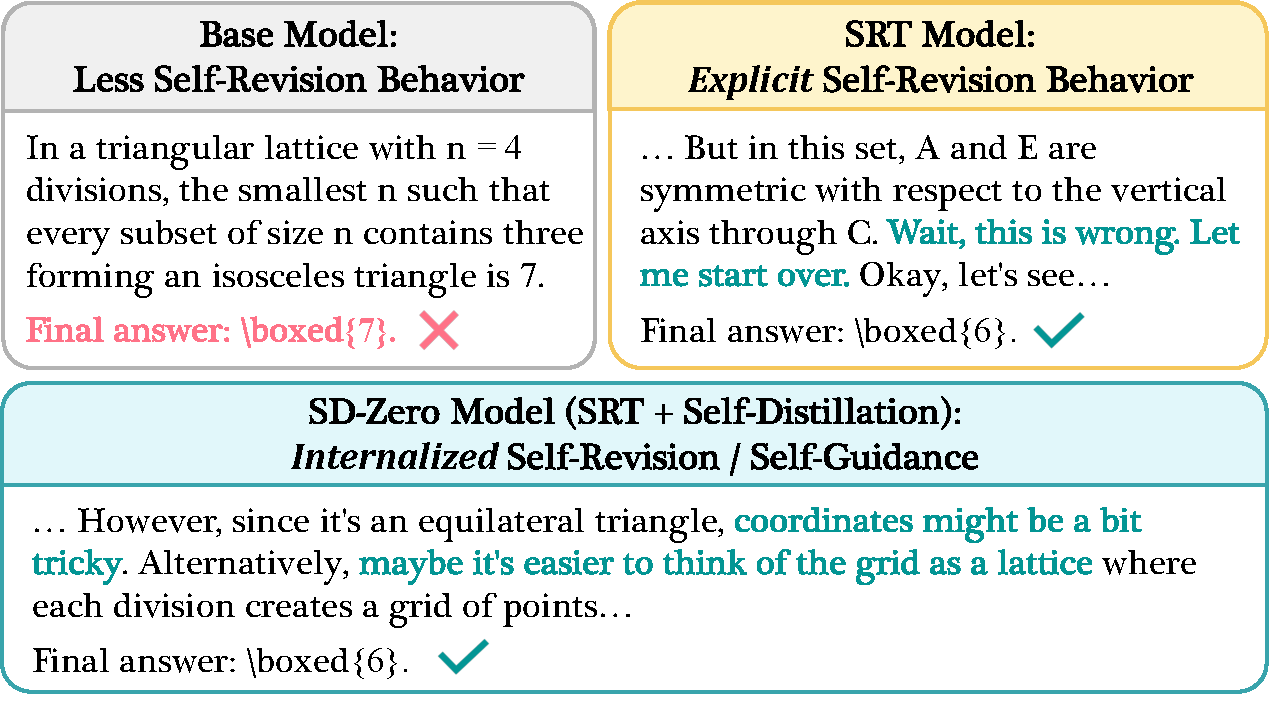
\includegraphics[width=\textwidth]{figures/Picture3.pdf}
    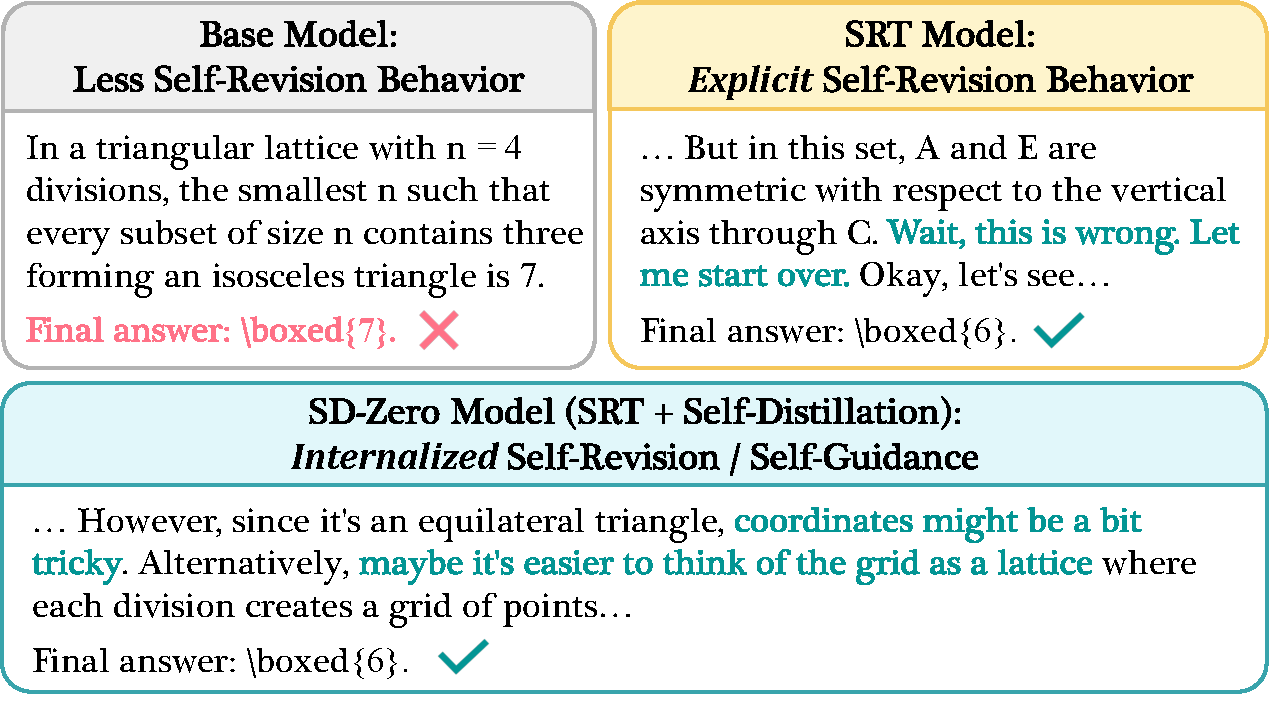
\includegraphics[width=0.57\textwidth]{figures/Picture3.pdf}
    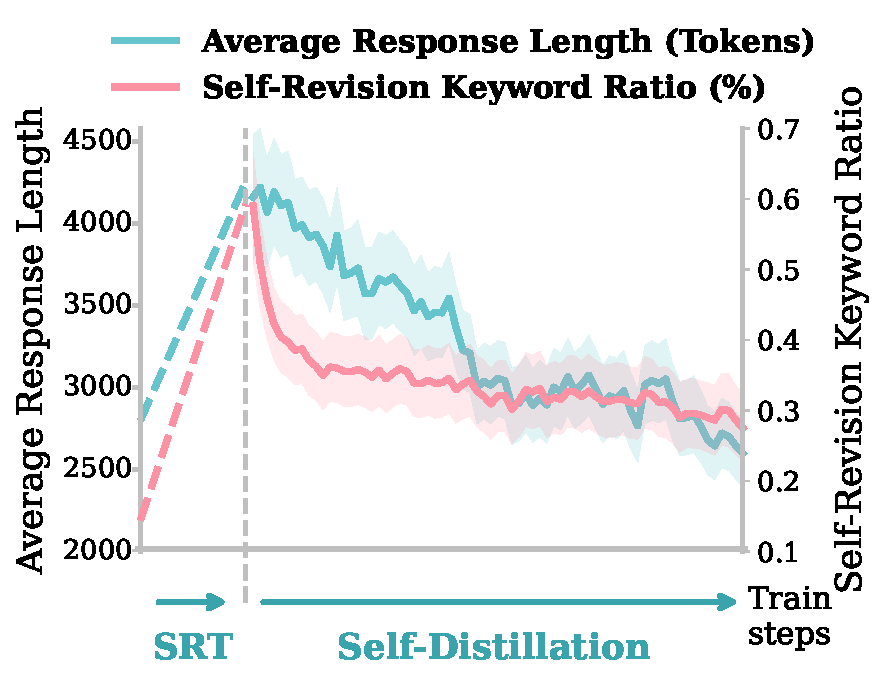
\includegraphics[width=0.42\textwidth,
    trim=0cm 0.1cm 0.1cm 0.4cm,
    clip
    ]{figures/publication_plot.pdf}
    \vspace{-1em}
    \captionsetup{font=small}
    \caption{\textbf{Evolution of self-revision behavior across training phases} for \qwen{} on \openmath{}. \textbf{Left:} Example reasoning traces from different model phases. The base model fails without revision, whereas the \sft{} model performs explicit self-revision and the \ours{} model exhibits more internalized self-guidance, identifying pitfalls and directing itself to the correct answer. \textbf{Right:} Training dynamics of self-revision behavior. Response length and explicit self-revision keywords rise during the SRT phase and fall during the \opsd{} phase, indicating a shift from overt revision to more internalized, token-efficient reasoning.}
    % \vspace{-10pt}
    \label{fig:behavior-evolution}
\end{figure}